\documentclass{book}

\usepackage[spanish]{babel}
\usepackage[utf8]{inputenc}

\usepackage{graphicx}
\usepackage{lipsum}
\usepackage{microtype}

\usepackage[T1]{fontenc}
\usepackage{lmodern}

\usepackage[pdftex]{hyperref}

\hypersetup{pdfauthor={J. S. Castellanos-Durán},pdftitle={RECANEWS Volumen 3 - Marzo 2015},colorlinks,linkcolor=black,urlcolor=blue}

\usepackage[paperwidth=210mm, paperheight=297mm, textwidth=160mm, textheight=240mm, bindingoffset=1cm]{geometry}


% obliczenie szerokości lewego marginesu
\usepackage{calc}
\newlength{\lmargin}
\setlength{\lmargin}{1in + \hoffset + \oddsidemargin}

\usepackage{flowfram}

\usepackage{color}

\usepackage{tikz}
\usepackage{anyfontsize}

% definicja ramek typu flow umieszczonych na stonie 1
\newflowframe[1]{8cm}{24\baselineskip}{-.50cm}{0\baselineskip}[frame1-1a]
\newflowframe[1]{8cm}{23\baselineskip}{8.5cm}{0\baselineskip}[frame1-2b]
%\newflowframe[1]{5cm}{27\baselineskip}{11cm}{0\baselineskip}[frame1-3c]

%definicja ramek statycznych wstawianych na stronie 1
\newstaticframe[1]{\paperwidth}{14cm}{-\lmargin}{12.5cm}[frameS-1a]
\newstaticframe[1]{14cm}{7\baselineskip}{0cm}{45\baselineskip}[frameS-1b]

%definicja ramki dymamicznej wstawiania na stonie nieparzystej
\newdynamicframe[odd]{2cm}{2cm}{-\lmargin}{6cm}[frameD-1a]
%definicja ramki dymamicznej wstawiania na stonie parzystej
\newdynamicframe[even]{2cm}{2cm}{\textwidth+\lmargin-2cm}{6cm}[frameD-1b]

% definicja ramek typu flow na kolejnych stronach
\newflowframe[>1]{8cm}{57\baselineskip}{-.50cm}{0\baselineskip}[frame2-1a]
\newflowframe[>1]{8cm}{57\baselineskip}{8.5cm}{0\baselineskip}[frame2-2a]
%\newflowframe[>1]{5cm}{57\baselineskip}{11cm}{0\baselineskip}[frame2-3a]

\definecolor{green}{rgb}{0.6,0.8,0.1}

\title{RECANEWS Volumen 3 - Marzo 2015}
\author{J. Sebastián Castellanos Durán}
\date{\relax}

\begin{document}

\pagestyle{empty}

% wstawienie numerów stron w ramki dynamiczne frameD-1a i frameD-1b
\begin{dynamiccontents*}{frameD-1a}
\begin{tikzpicture}
\draw(0,0) node [fill=orange, minimum width=2cm, minimum height=2cm]{
{\sffamily\bfseries\Huge\color{white}\thepage}
};
\end{tikzpicture}
\end{dynamiccontents*}

\begin{dynamiccontents*}{frameD-1b}
\begin{tikzpicture}
\draw(0,0) node [fill=orange, minimum width=2cm, minimum height=2cm]{
{\sffamily \bfseries\Huge\color{white}\thepage}
};
\end{tikzpicture}
\end{dynamiccontents*}


% wstawienie grafiki w ramkię statyczną frameS-1a
\begin{staticcontents*}{frameS-1a}
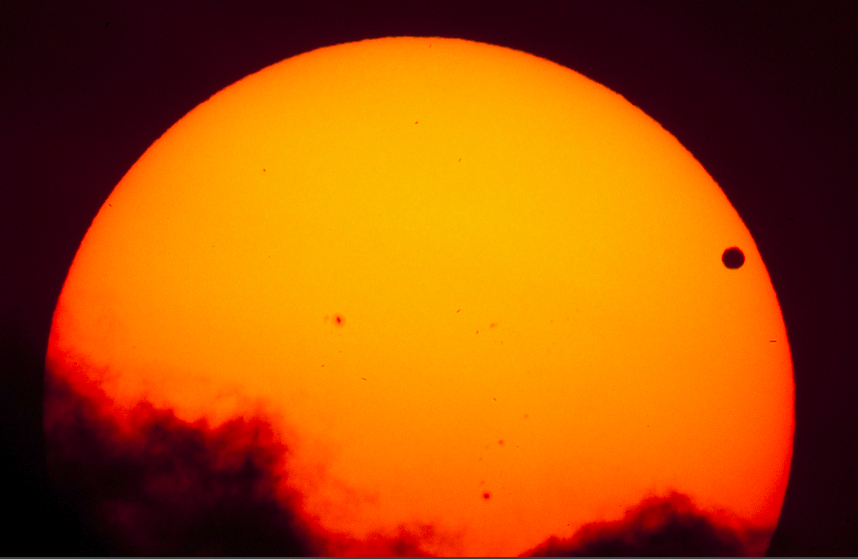
\includegraphics[width=1\textwidth]{fig11.jpg}
\end{staticcontents*}

% wypełnienie tekstem ramki statycznej frameS-1b
\begin{staticcontents*}{frameS-1b}
\begin{tikzpicture}
\draw(0,0) node [fill=white, text width=13cm, inner sep=5mm, opacity=0.7]{
\large\sffamily
{\fontsize{70}{30}\selectfont {\color{black} RECANEWS}}\\


{\fontsize{30}{30}\selectfont {\color{black} Volumen 3}}\\
\begin{center}
{\fontsize{30}{30}\selectfont {\color{black} Llamada a publicaciones}}\\
\end{center}
\begin{flushright}
{\fontsize{30}{30}\selectfont {\color{black} Marzo 2015}}
\end{flushright}
};
\end{tikzpicture}
\end{staticcontents*}


%\tableofcontents{}
% wlanie tekstu do wszystkich ramek typu flow



\newpage


\renewcommand\thesection{\arabic{section}}
\renewcommand\thesubsection{\arabic{subsection}}


%*********************************************
\addcontentsline{toc}{section}{}
\section*{}
%*********************************************


¿Quieres hacer un Ph.D?


... we have a field of understandably disgruntled young people with PhDs but no realistic prospect of ever earning a settled living working in the field they have prepared for. This problem has worsened considerably in recent  years as the number of postdoctoral positions has almost halved since 2006. New PhDs have to battle it out with existing postdoctoral researchers for the meagre supply of suitable jobs. It’s a terrible situation.

https://telescoper.wordpress.com/2015/02/19/science-produces-too-many-phds/

%*********************************************
\addcontentsline{toc}{section}{}
\section*{}
%*********************************************

La UIS, Bucaramanga en la colaboración Auger 

%*********************************************
\addcontentsline{toc}{section}{}
\section*{}
%*********************************************



Les comparto un articulo que escribí dentro de la colaboración Planck y envié a A\&A recientemente.
Va sobre el estudio del rol de campo magnético en la formación de estructuras en el ISM a partir de las observaciones de la emisión termica polarizada del polvo interestelar que hizo el observatorio espacial Planck.
Sus comentarios son bienvenidos!

http://arxiv.org/abs/1502.04123

%*********************************************
\addcontentsline{toc}{section}{}
\section*{}
%*********************************************


Astronomía al Aire, una cita con el Cielo
La noche, los astros, el universo han ejercido una fascinación persistente en hombres y mujeres a través de los tiempos.
Astronomía al Aire busca apoyarse en esa fascinaciónpara contribuir a crear una cultura científica. Crear curiosidad por el diverso mundo
de la astrofísica, de lo que sabemos, de lo que ignoramos.

Una serie de micros radiales usa el poder de penetración de la radio para seducir al oyente.  Todos los días a través de  UIS AM- 670KHz a las 7:00 a.m. 12:30 p.m y 5:30 p.m podrán escuchar un apasionante tema semanal. Esta semana se conversa sobre los agujeros negros, el triunfo de la gravedad.

Un blog http://halley.uis.edu.co/aire/ les da permanencia y los complementa preservando el audio y planteando preguntas.  En el blog el visitante puede puede oír los micros, leer los textos y formular comentarios, preguntas e inquietudes que serán respondidas en línea, a través @AstroAlAire y astronomia.al.aire@uis.edu.co .


Un programa radial más largo con invitados, permitirá ampliar los temas y mantener el interés de los oyentes..

Astronomía al Aire deriva de los esfuerzos que el Grupo Halley ha venido desarrollando a lo largo de varios lustros en la promoción de la Astronomía
en el Nororiente colombiano.

Es posible gracias al profesionalismo de TeleUIS Comunicaciones, al respaldo entusiasta de la Vicerrectoría de Investigación de la Universidad Industrial de Santander y al apoyo irrestricto de la Escuela de Física. Está coordinada por Héctor Rago y Luis Núnez.

%*********************************************
\addcontentsline{toc}{section}{}
\section*{}
%*********************************************

El Dr. Oscar Leonardo Ramírez Suárez fue contratado desde Enero como Docente Investigador en la Universidad ECCI. Es Físico de la U. Nacional, donde hizo su pregrado en Física Nuclear en el Centro Internacional de Física. Luego estudió su MSc en el Instituto Balseiro en Argentina en Física de Altas Energías, becado por el ICTP. Posteriormente hizo su doctorado en la U. Libre de Bruselas en Física Nuclear. Su área principal de investigación es en modelos teóricos de reacciones nucleares aplicados a astrofísica. Tiene colaboraciones activas con la ULB (Bélgica) y el CIF (Colombia). En la UECCI trabajará con el grupo de Ciencias Básicas conformado por Germán Chaparro, Oscar Restrepo y co-investigadores, apoyando también las líneas de investigación de Radioastronomía y Astroestadística.

Germán Chaparro Molano, PhD

%*********************************************
\addcontentsline{toc}{section}{}
\section*{}
%*********************************************


http://www.astrosen.unam.mx/~verano/

de Katherine Mafla

%*********************************************
\addcontentsline{toc}{section}{}
\section*{}
%*********************************************

Ya están abiertas las inscripciones al posgrado (Maestría, Doctorado) de Física en Uniandes donde el grupo de astrofísica puede ofrecer temas de investigación. La fecha límite es el 28 de Abril.

Este año aparte de la posibilidad de apoyo financiero a través de asistencias graduadas también hay becas de Colciencias (para personas que ya tengan una maestría).

Si les interesa saber más sobre los detalles pueden escribirme un correo a je.forero@uniandes.edu.co


El 4 de marzo habrá una charla informativa sobre posgrados en Uniandes (programas, fuentes de financiación, etc).

Los invito para que los interesados se inscriban y asistan:
http://goo.gl/UfPi3q


Gracias y saludos,

Jaime

%*********************************************
\addcontentsline{toc}{section}{}
\section*{}
%*********************************************

The Yale University Astronomy Department is pleased to invite applications for the second annual Hoffleit Undergraduate Astronomy Research Scholarship. This program serves as an opportunity for keen undergraduates in STEM fields with a strong interest in pursuing astronomy to spend 6-8 weeks performing research with Yale astronomers. Research topics cover a wide range, from the characterization and discovery of exoplanets, the study of the Sun and stars, to the origin and evolution of small and large galaxies. Yale’s astronomy department is located in New Haven, CT, near historic downtown and the East Rock neighborhood. New Haven is a vibrant city in the summertime; home to the Arts and Ideas festival, as well as many cafes and restaurants. The undergraduate students will be housed together in the beautiful campus residential colleges where they will have the opportunity to interact with undergraduate scholars from other departments.

The program encourages undergraduates from all nationalities to apply, particularly those with a strong desire to continue to graduate school.


To apply or find out more, visit\\ \url{http://goo.gl/sYbj6H}\\

The fellowship is named in honor of Dr. E. Dorrit Hoffleit, was a senior research astronomer at Yale for more than fifty years in the University’s Department of Astronomy.

Louise Edwards, PhD

%*********************************************
\addcontentsline{toc}{section}{}
\section*{}
%*********************************************

Charlas Spacio

\begin{description}
\item[Marzo 7 - 4:00pm:] ​Influencia de rotación y outflows en Lyman Alpha Emitters\\
 ​Maria Camila Remolina\\
 Uniandes.
\item[Marzo 7 - 5:15pm:]​ Modelos de Formación Estelar en Simulaciones de Galaxias\\
Luis Fernando Quiroga\\
 Universidad de Antioquia.​ (Skype)
\item[Marzo 14 - 4:00pm:]  ¿​Una secuencia principal de galaxias?\\ 
Juan Rafael Martinez Galarza\\ 
Harvard-Smithsonian Center for Astrophysics. ​(Skype)
\item[Marzo 14 - 5:15pm:] Magneto no es un héroe: campos magnéticos y la formación de estrellas\\ 
 ​Juan Diego Soler\\
 Instituto de Astrofísica Paris. ​(Skype)  
\item[Marzo 21 - 4:00pm:] ​Geología y Astrobiología​\\ 
Julian Corzo\\  
UNAL
\item[Marzo 21 - 5:15pm:] ​S​ociología y Materia Oscura\\
​Paola Castaño\\ 
UniAndes  
\item[Marzo 28 - 4:00pm:]  ​Las galaxias satélite y su extraña distribución espacial\\
Veronica Arias\\
UniAndes.
\item[Marzo 28 - 5:15pm:]  ​Asociaciones de Galaxias Enanas en el Grupo Local\\
​Juan Nicolas Garavito\\
UniAndes 
\end{description}


%*********************************************
\addcontentsline{toc}{section}{}
\section*{}
%*********************************************

COCOA Libro de resumenes

%*********************************************
\addcontentsline{toc}{section}{}
\section*{}
%*********************************************

COCOA Publicación memorias

%*********************************************
%*********************************************
\addcontentsline{toc}{section}{¿Cómo publicar en RECANEWS?}
\section*{¿Cómo publicar en RECANEWS?}
%*********************************************

Para publicar en RECANEWS se debe enviar un correo a reca.news@gmail.com con las siguientes especificaciones:
\begin{description}
\item[Correo:]\url{reca.news@gmail.com}
\item[Asunto:]Título de la publicación
\item[Contenido:]Contenido de la publicación\\
Persona encargada (Opcional)\\
Correo de la persona encargada (Opcional)
\end{description}
  
%*********************************************
\addcontentsline{toc}{section}{Repositorio de RECANEWS}
\section*{Repositorio de RECANEWS}
%*********************************************

Repositorio: \url{https://github.com/recanews}\\



%*********************************************
\addcontentsline{toc}{section}{Contacto del RECA}
\section*{Contacto del RECA:}
%*********************************************

\begin{description}
\item[Correo RECA:]\url{reca.astronomia@gmail.com}
\item[Facebook:] \url{https://www.facebook.com/RECAstronomia}
\item[Google$+$:] \url{http://goo.gl/P0DEf4}
\item[Twitter:] \url{https://twitter.com/RECAstronomia}
\item[Pagina Web:] \url{http://goo.gl/Fl4zQP}
\end{description}


%*********************************************
\addcontentsline{toc}{section}{Representantes de RECA en las regiones}
\section*{Representantes de RECA en las regiones}
%*********************************************
\begin{description}
\item[Medellín:]Malory Agudelo Vásquez\\
\url{magudelov@gmail.com}\\ \url{magudelov@fisica.udea.edu.co}
\item[Pereira:]Luisa Fernanda Cardona\\ \url{luisferncardona@utp.edu.co}
\item[Pasto:]Katherine Mafla Oliva\\
\url{skmofis13@gmail.com}
\item[Cali:]Daniel Santacruz\\
\url{santacruz121@gmail.com}
\item[Bogotá:]Maria Camila Remolina Gutierrez\\
\url{mc.remolina197@uniandes.edu.co}\\

Andres Felipe Ramos Padilla\\
\url{andresrp25@gmail.com}\\

Juan David Jimenez Nieto\\
\url{jdjimenezn@correo.udistrital.edu.co}
\end{description}


%*********************************************
\addcontentsline{toc}{section}{Editor RECANEWS}
			\section*{Editor RECANEWS}
%********************************************
  
\begin{flushright}
J. Sebastián Castellanos-Durán\\
\url{jsebastian405@gmail.com}
\end{flushright}
\begin{flushright}
Cualquier comentario por favor escribir al correo  \url{reca.news@gmail.com}\\
Marzo 2015
\end{flushright}


\end{document}


